% ============================================================
%  Chapter 13: Quadratic Programming
%  Algorithms for Optimization, 2nd ed. (Kochenderfer & Wheeler, 2026)
%  Beamer slides --- Python equivalents of all Julia code
% ============================================================
\documentclass[aspectratio=169,10pt]{beamer}

\usetheme{Madrid}
\usecolortheme{seahorse}

\usepackage{amsmath,amssymb,bm}
\usepackage{mathtools}
\usepackage{graphicx}
\usepackage{listings}
\usepackage{xcolor}
\usepackage{booktabs}
\usepackage{tikz}
\usetikzlibrary{arrows.meta,positioning,shapes.geometric}

\graphicspath{{figures/}}

% -- Python listing style ------------------------------------------------------
\definecolor{codegreen}{rgb}{0.0,0.5,0.2}
\definecolor{codegray}{rgb}{0.5,0.5,0.5}
\definecolor{codepurple}{rgb}{0.5,0.0,0.5}
\lstset{
  language=Python,
  basicstyle=\ttfamily\scriptsize,
  numbers=left,
  numberstyle=\tiny\color{codegray},
  numbersep=5pt,
  frame=single,
  backgroundcolor=\color{gray!7},
  keywordstyle=\color{blue}\bfseries,
  commentstyle=\color{codegreen},
  stringstyle=\color{codepurple},
  breaklines=true,
  showstringspaces=false,
  tabsize=4,
  captionpos=b,
}

\setbeamertemplate{footline}[frame number]
\setbeamertemplate{navigation symbols}{}

% -- Math operators ------------------------------------------------------------
\DeclareMathOperator*{\minimize}{minimize}
\DeclareMathOperator*{\maximize}{maximize}

% -- Macros --------------------------------------------------------------------
\newcommand{\bx}{\mathbf{x}}
\newcommand{\bq}{\mathbf{q}}
\newcommand{\bb}{\mathbf{b}}
\newcommand{\bA}{\mathbf{A}}
\newcommand{\bB}{\mathbf{B}}
\newcommand{\bG}{\mathbf{G}}
\newcommand{\bh}{\mathbf{h}}
\newcommand{\bc}{\mathbf{c}}
\newcommand{\bC}{\mathbf{C}}
\newcommand{\bd}{\mathbf{d}}
\newcommand{\bQ}{\mathbf{Q}}
\newcommand{\bU}{\mathbf{U}}
\newcommand{\bV}{\mathbf{V}}
\newcommand{\bT}{\mathbf{T}}
\newcommand{\bE}{\mathbf{E}}
\newcommand{\bmu}{\boldsymbol{\mu}}
\newcommand{\blambda}{\boldsymbol{\lambda}}
\newcommand{\R}{\mathbb{R}}
\newcommand{\norm}[1]{\left\|#1\right\|}

% =============================================================================
\title[Ch.~13: Quadratic Programming]{Chapter 13: Quadratic Programming}
\subtitle{Algorithms for Optimization, 2nd Edition}
\author{Kochenderfer \& Wheeler (2026)}
\date{Lecture Slides}
\institute{MIT Press}

\begin{document}

\begin{frame}
  \titlepage
\end{frame}

% -- Outline -------------------------------------------------------------------
\begin{frame}{Chapter Overview}
  \tableofcontents
\end{frame}

\AtBeginSection[]{
  \begin{frame}{Outline}
    \tableofcontents[currentsection]
  \end{frame}
}

% =============================================================================
\section{13.1 Problem Formulation}
% =============================================================================

\begin{frame}{What Is a Quadratic Program?}
  \begin{block}{Quadratic Program (General Form) --- Eq.~(13.1)}
    \[
      \minimize_{\bx}\quad \frac{1}{2}\bx^{\top}\bQ\bx + \bq^{\top}\bx
      \quad\text{subject to}\quad
      \bC_{\text{LE}}\bx \leq \bd_{\text{LE}},\quad
      \bC_{\text{EQ}}\bx = \bd_{\text{EQ}}
    \]
    \medskip
    \begin{tabular}{ll}
      $\bQ \in \R^{n\times n}$ & symmetric cost matrix (Hessian of objective)\\
      $\bq \in \R^n$           & linear cost vector (gradient term)\\
      $\bC_{\text{LE}},\bd_{\text{LE}}$ & linear inequality constraints\\
      $\bC_{\text{EQ}},\bd_{\text{EQ}}$ & linear equality constraints\\
    \end{tabular}
  \end{block}

  \begin{itemize}
    \item $\frac{1}{2}\bx^{\top}\bQ\bx$ contributes quadratic components
          $\tfrac{1}{2}Q_{ii}x_i^2$ and product components
          $(\tfrac{1}{2}Q_{ij}+\tfrac{1}{2}Q_{ji})x_ix_j$ for $i<j$
    \item \textbf{Connection to Newton's method:} second-order Taylor approximation
          about $\bx_{\text{ref}}$ gives $\bQ = \nabla^2 f(\bx_{\text{ref}})$,
          $\bq = \nabla f(\bx_{\text{ref}})$
    \item QP = Newton's method subject to linear constraints
  \end{itemize}
\end{frame}

\begin{frame}{Convex QP $\Leftrightarrow$ Least-Squares Problem}
  \begin{block}{Conversion via Cholesky --- Eq.~(13.2)}
    When $\bQ$ is \textbf{positive definite}, factor $\bQ = \bU^{\top}\bU$ (Cholesky).
    Then the QP becomes the \emph{least-squares problem}:
    \[
      \minimize_{\bx}\; \norm{\bA\bx - \bb}
      \quad\text{s.t.}\quad
      \bC_{\text{LE}}\bx \leq \bd_{\text{LE}},\;
      \bC_{\text{EQ}}\bx = \bd_{\text{EQ}}
    \]
    with $\bA = \bU$ and $\bb = -\bU^{-\top}\bq$.
  \end{block}

  \begin{columns}[T]
    \column{0.48\textwidth}
      \textbf{Transformation chain} (Fig.~13.1):
      \begin{center}
        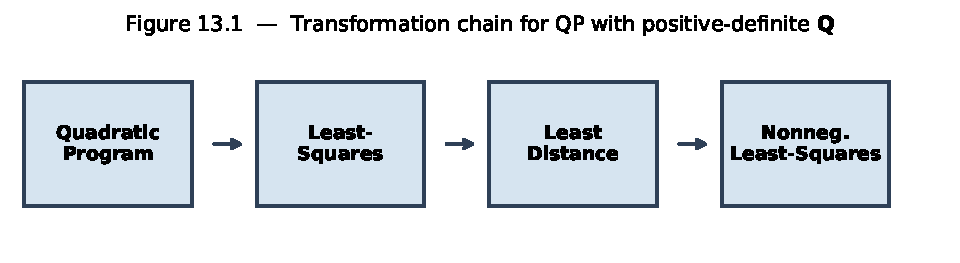
\includegraphics[width=\linewidth]{fig_transform_chain}
      \end{center}

    \column{0.48\textwidth}
      \textbf{Key observations:}
      \begin{itemize}
        \item Feasible set = convex polytope (same as LP)
        \item Solution need \emph{not} lie at a vertex
        \item May be interior, boundary, infeasible, or unbounded
      \end{itemize}
  \end{columns}
\end{frame}

\begin{frame}{Example 13.1 --- QP with Elliptical Contours}
  \begin{columns}[T]
    \column{0.50\textwidth}
      \begin{block}{Problem}
        \[
          \minimize_{x_1,x_2}
          \left\|\begin{bmatrix}2&1\\-4&3\end{bmatrix}
          \begin{bmatrix}x_1\\x_2\end{bmatrix}
          - \begin{bmatrix}1\\2\end{bmatrix}\right\|
        \]
        \[
          \text{s.t.}\quad
          2x_1 - x_2 \geq 2,\quad
          x_1 - 3x_2 \leq 4
        \]
      \end{block}
      \begin{itemize}
        \item Objective forms elliptical contours
        \item Center of ellipses may lie \emph{outside} feasible set
        \item \textbf{Solution:} $\bx^* = [1.4,\; 0.8]^{\top}$
        \item Solution on boundary, not at vertex
      \end{itemize}

    \column{0.46\textwidth}
      \begin{center}
        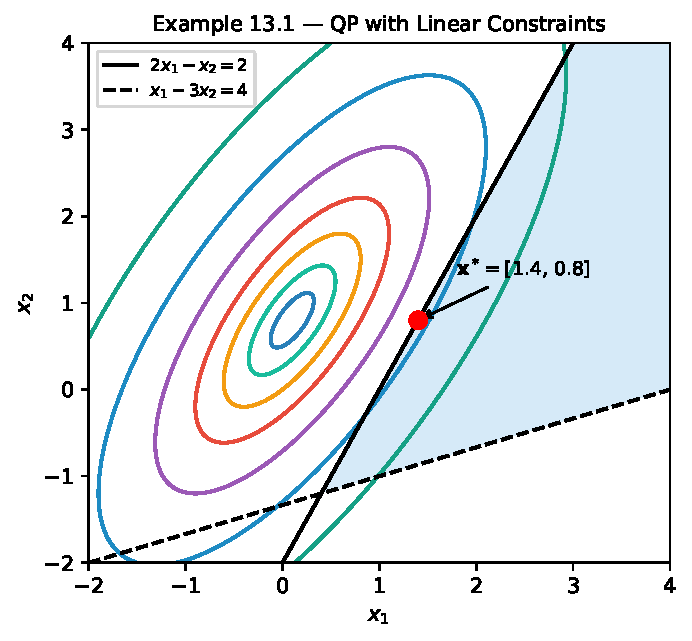
\includegraphics[width=\linewidth]{fig_qp_example}
      \end{center}
  \end{columns}
\end{frame}

\begin{frame}{Four Solution Cases for a QP}
  \begin{center}
    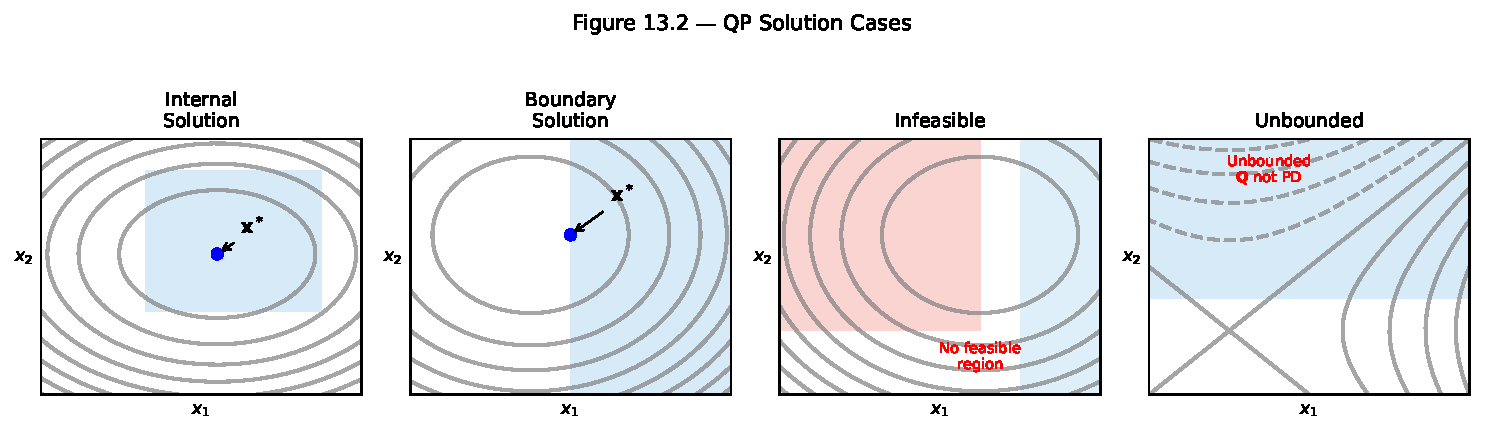
\includegraphics[width=0.92\linewidth]{fig_qp_cases}
  \end{center}
  \begin{itemize}
    \item \textbf{Internal:} unconstrained minimizer is inside feasible set
    \item \textbf{Boundary:} minimizer is on the boundary of the feasible set
    \item \textbf{Infeasible:} feasible set is empty
    \item \textbf{Unbounded:} $\bQ$ is not positive definite $\Rightarrow$ may be unbounded
  \end{itemize}
\end{frame}

% =============================================================================
\section{13.2 Unconstrained Least-Squares Problems}
% =============================================================================

\begin{frame}{Unconstrained Least Squares}
  \begin{block}{Problem Statement --- Eq.~(13.3)}
    \[
      \minimize_{\bx}\; \norm{\bA\bx - \bb},
      \quad \bA \in \R^{m\times n},\; \bx \in \R^n,\; \bb \in \R^m
    \]
  \end{block}

  \vspace{0.3em}
  \begin{columns}[T]
    \column{0.48\textwidth}
      \textbf{Case 1: $\bA$ invertible} \hfill Eq.~(13.4)
      \[
        \bx^* = \bA^{-1}\bb
      \]
      Unique solution; objective = 0.

      \vspace{0.5em}
      \textbf{Case 2: $\bA$ not invertible} --- use SVD:
      \[
        \bA = \bU\begin{bmatrix}\bT & \mathbf{0}\\\mathbf{0}&\mathbf{0}\end{bmatrix}\bV^{\top}
        \quad\text{Eq.~(13.5)}
      \]
      where $\bU \in \R^{m\times m}$, $\bV \in \R^{n\times n}$ orthogonal,
      $\bT \in \R^{k\times k}$ diagonal (positive).

    \column{0.48\textwidth}
      \textbf{Minimum-norm solution via pseudoinverse:}
      \begin{align}
        \bx^* &= \bA^+\bb \tag{13.18}\\[4pt]
        \bA^+ &= \bV\begin{bmatrix}\bT^{-1}&\mathbf{0}\\\mathbf{0}&\mathbf{0}\end{bmatrix}\bU^{\top}
        \tag{13.19}
      \end{align}

      \vspace{0.5em}
      \textbf{Special forms:}
      \begin{align}
        \bA^+ &= (\bA^{\top}\bA)^{-1}\bA^{\top}
          & &\text{cols indep.} \tag{13.20}\\
        \bA^+ &= \bA^{\top}(\bA\bA^{\top})^{-1}
          & &\text{rows indep.} \tag{13.21}\\
        \bA^+ &= \bA^{-1}
          & &\bA\text{ invertible} \tag{13.22}
      \end{align}
  \end{columns}
\end{frame}

\begin{frame}{SVD Derivation of the Pseudoinverse}
  Substituting SVD into $\norm{\bA\bx - \bb}^2$:
  \begin{align}
    \norm{\bA\bx - \bb}^2
    &= \left\|\bU\begin{bmatrix}\bT&\mathbf{0}\\\mathbf{0}&\mathbf{0}\end{bmatrix}
       \bV^{\top}\bx - \bb\right\|^2 \tag{13.6} \\[4pt]
    &= \left\|\begin{bmatrix}\bT&\mathbf{0}\\\mathbf{0}&\mathbf{0}\end{bmatrix}
       (\bV^{\top}\bx) - (\bU^{\top}\bb)\right\|^2 \tag{13.8}\\[4pt]
    &= \norm{\bT\mathbf{v}_{\text{fixed}} - \bU_1^{\top}\bb}^2
       + \norm{\bU_2^{\top}\bb}^2 \tag{13.11}
  \end{align}

  where $\bU = [\bU_1, \bU_2]$, $\bV = [\bV_1, \bV_2]$,
  $\mathbf{v}_{\text{fixed}} = \bV_1^{\top}\bx$.

  \begin{block}{Optimal Fixed Component --- Eq.~(13.13)}
    \[
      \mathbf{v}^*_{\text{fixed}} = \bT^{-1}\bU_1^{\top}\bb
    \]
    \begin{itemize}
      \item $\mathbf{v}_{\text{free}} = \bV_2^{\top}\bx$ is unconstrained; setting it to $\mathbf{0}$
            gives the \textbf{minimum-norm} solution.
      \item Result: $\bx^* = \bV\begin{bmatrix}\bT^{-1}&\mathbf{0}\\\mathbf{0}&\mathbf{0}\end{bmatrix}\bU^{\top}\bb = \bA^+\bb$
    \end{itemize}
  \end{block}
\end{frame}

\begin{frame}[fragile]{Python: Pseudoinverse \& Least Squares}
\begin{lstlisting}[caption={Unconstrained least-squares via pseudoinverse (NumPy/SciPy)}]
import numpy as np
from scipy.linalg import lstsq, svd

# Example: A is 3x2 (overdetermined), b is 3-vector
A = np.array([[2., 1.],
              [-4., 3.],
              [1., 1.]])
b = np.array([1., 2., 0.5])

# --- Method 1: pseudoinverse via SVD ---
A_pinv = np.linalg.pinv(A)      # V T^{-1} U^T (eq. 13.19)
x_star = A_pinv @ b
print(f"x* (pinv): {x_star}")   # minimum-norm least-squares solution

# --- Method 2: scipy lstsq (numerically robust, recommended) ---
x_lstsq, residuals, rank, sv = lstsq(A, b)
print(f"x* (lstsq): {x_lstsq}")

# --- Method 3: normal equations (columns linearly independent) ---
x_normal = np.linalg.solve(A.T @ A, A.T @ b)  # eq. (13.20)
print(f"x* (normal eq): {x_normal}")

# Verify residual
print(f"||Ax - b|| = {np.linalg.norm(A @ x_star - b):.6f}")
\end{lstlisting}
\end{frame}

% =============================================================================
\section{13.3 Least Squares with Linear Inequalities}
% =============================================================================

\begin{frame}{Least Squares with Linear Inequalities}
  \begin{block}{Problem Statement --- Eq.~(13.23)}
    \[
      \minimize_{\bx}\; \norm{\bA\bx - \bb}
      \qquad \text{subject to}\quad \bC\bx \geq \bd
    \]
    (Less-than inequalities are negated; equality constraints are eliminated.)
  \end{block}

  \vspace{0.3em}
  \textbf{Equality constraint elimination via LQ decomposition:}
  \begin{enumerate}
    \item Decompose $\bC_{\text{EQ}} = \mathbf{L}\mathbf{Q}$ (LQ = QR of transpose)
    \item Substitute $\bx = \mathbf{Q}^{\top}\begin{bmatrix}\mathbf{y}_1^*\\\mathbf{y}_2\end{bmatrix}$
          where $\mathbf{y}_1^* = \mathbf{L}_{11}^{-1}\bd_{\text{EQ}}$ \hfill Eq.~(13.24)
    \item Optimization reduces to variable $\mathbf{y}_2$:
  \end{enumerate}

  \begin{block}{Reduced Problem --- Eq.~(13.26)}
    \[
      \minimize_{\mathbf{y}_2}\;
      \left\|(\bA\mathbf{Q}^{\top})_{(\cdot,c+1:n)}\mathbf{y}_2
      - \left(\bb - (\bA\mathbf{Q}^{\top})_{(\cdot,1:c)}\mathbf{y}_1^*\right)\right\|
    \]
    \[
      \text{s.t.}\quad
      (\bC\mathbf{Q}^{\top})_{(\cdot,c+1:n)}\mathbf{y}_2
      \geq \bd - (\bC\mathbf{Q}^{\top})_{(\cdot,1:c)}\mathbf{y}_1^*
    \]
  \end{block}
\end{frame}

\begin{frame}{Algorithm 13.1 --- Solve Quadratic Program (General Form)}
  \begin{alertblock}{Method}
    Convert QP $\to$ LeastSquaresWithInequalities, solve, back-substitute.
    Assumes $\bC_{\text{EQ}} \in \R^{c\times n}$ has rank $c < n$.
  \end{alertblock}

  \textbf{Steps:}
  \begin{enumerate}
    \item Extract $\bA, \bb, \bC_{\text{LE}}, \bd_{\text{LE}}, \bC_{\text{EQ}}, \bd_{\text{EQ}}$
    \item Compute LQ decomposition: $\bC_{\text{EQ}} = \mathbf{L}\mathbf{Q}$
    \item Compute $\mathbf{y}_1^* = \mathbf{L}_{11}^{-1}\bd_{\text{EQ}}$
    \item Form reduced matrices $\bA_2 = (\bA\mathbf{Q}^{\top})_{(\cdot,c+1:n)}$, etc.
    \item Solve LeastSquaresWithInequalities for $\mathbf{y}_2$
    \item Return $\bx^* = \mathbf{Q}^{\top}[\mathbf{y}_1^*;\, \mathbf{y}_2]$
  \end{enumerate}

  \begin{columns}[T]
    \column{0.58\textwidth}
    \begin{exampleblock}{Complexity}
      \begin{itemize}
        \item LQ decomposition: $O(cn^2)$
        \item Reduced problem size: $(n-c)$ variables
        \item Overall cost dominated by inner NNLS solver
      \end{itemize}
    \end{exampleblock}

    \column{0.38\textwidth}
    \textbf{Key assumption:} $\bC_{\text{EQ}}$ is full row rank (no redundant/contradictory equality constraints).
  \end{columns}
\end{frame}

\begin{frame}{Example 13.2 --- 3D QP with Equality Constraint}
  \begin{columns}[T]
    \column{0.50\textwidth}
      \begin{block}{Original 3D Problem}
        \small
        \[
          \minimize_{\bx}
          \left\|\begin{bmatrix}1&2&3\\-2&0&0\end{bmatrix}\bx
          - \begin{bmatrix}1\\2\end{bmatrix}\right\|
        \]
        \[
          \bx \leq \begin{bmatrix}1\\1\\1\end{bmatrix}\!,\;
          \bx \geq \mathbf{0},\;
          [-1\ \ 1\ \ 1]\bx = 0
        \]
        Feasible region: $0\leq x_1\leq 1$, $0\leq x_3\leq 1$, $x_2 = x_3$
      \end{block}
      \textbf{Solution:} $\bx^* = [0,\; 0.2,\; 0.2]^{\top}$

      After equality elimination: $\mathbf{y}_1 = [0]$, reduced to 2D problem.

    \column{0.46\textwidth}
      \begin{center}
        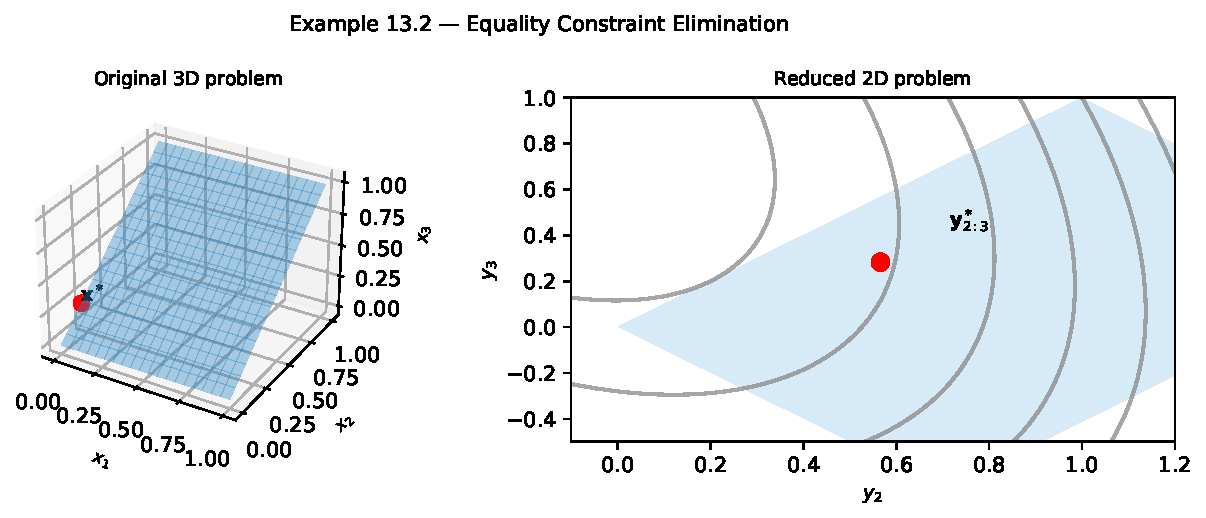
\includegraphics[width=\linewidth]{fig_example13_2}
      \end{center}
  \end{columns}
\end{frame}

\begin{frame}[fragile]{Python: Least Squares with Inequalities}
\begin{lstlisting}[caption={Algorithm 13.1 implemented with SciPy (quadratic program solver)}]
import numpy as np
from scipy.optimize import minimize

def solve_qp_lstsq(A, b, C_LE, d_LE, C_EQ=None, d_EQ=None):
    """Solve minimize||Ax - b|| s.t. C_LE x <= d_LE, C_EQ x = d_EQ"""
    n = A.shape[1]
    # Objective: minimize (1/2)||Ax - b||^2
    Q = A.T @ A           # = U^T U  (eq 13.1 with q = -A^T b)
    q = -A.T @ b

    constraints = []
    if C_LE is not None:
        # C_LE x <= d_LE  =>  -(C_LE x - d_LE) >= 0
        constraints.append({'type': 'ineq',
                            'fun': lambda x: d_LE - C_LE @ x})
    if C_EQ is not None:
        constraints.append({'type': 'eq',
                            'fun': lambda x: C_EQ @ x - d_EQ})

    def obj(x):
        return 0.5 * x @ Q @ x + q @ x

    def grad(x):
        return Q @ x + q

    res = minimize(obj, np.zeros(n), jac=grad,
                   method='SLSQP', constraints=constraints)
    return res.x, res.success

# Example 13.1
A = np.array([[2., 1.], [-4., 3.]])
b = np.array([1., 2.])
C_LE = np.array([[-2., 1.], [1., -3.]])  # >= form negated
d_LE = np.array([-2., 4.])
x_star, ok = solve_qp_lstsq(A, b, C_LE, d_LE)
print(f"x* = {x_star.round(4)}")  # Expected: [1.4, 0.8]
\end{lstlisting}
\end{frame}

% =============================================================================
\section{13.4 Least Distance Programming}
% =============================================================================

\begin{frame}{Least Distance Programming}
  \begin{block}{Least Distance Program (LDP) --- Eq.~(13.27)}
    \[
      \minimize_{\bx}\; \norm{\bx}
      \qquad \text{subject to}\quad \bG\bx \geq \bh
    \]
    where $\bG \in \R^{m\times n}$, $\bx \in \R^n$, $\bh \in \R^m$.\\
    Find the point in the feasible set \textbf{closest to the origin}.
  \end{block}

  \begin{columns}[T]
    \column{0.50\textwidth}
      \begin{center}
        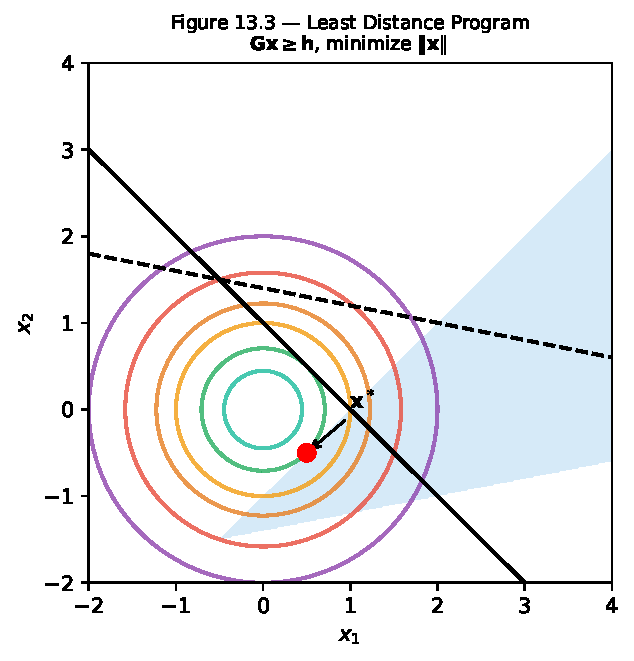
\includegraphics[width=0.9\linewidth]{fig_least_distance}
      \end{center}

    \column{0.46\textwidth}
      \textbf{Reduction from Least Squares with Inequalities:}
      \begin{enumerate}
        \item Apply SVD: $\bA = \bU\begin{bmatrix}\bT&\mathbf{0}\\\mathbf{0}&\mathbf{0}\end{bmatrix}\bV^{\top}$
        \item Objective becomes $\norm{\bT\mathbf{v}_{\text{fixed}} - \bU_1^{\top}\bb}^2$
        \item Change of variables: $\mathbf{z} = \bT\mathbf{v}_{\text{fixed}} - \bU_1^{\top}\bb$
        \item Minimizing $\norm{\mathbf{z}}$ subject to linear inequalities \hfill Eq.~(13.29--13.31)
      \end{enumerate}
      \vspace{0.5em}
      \textbf{Properties:}
      \begin{itemize}
        \item LDP is \emph{not always feasible}
        \item Solution is \emph{unique} if it exists
      \end{itemize}
  \end{columns}
\end{frame}

\begin{frame}{LDP $\to$ NNLS Transformation}
  The LDP can be solved via a \textbf{nonnegative least-squares} (NNLS) problem:

  \begin{block}{NNLS Form --- Eq.~(13.32--13.33)}
    \[
      \minimize_{\bx}\; \norm{\bE\bx - \mathbf{f}}
      \qquad \text{subject to}\quad \bx \geq \mathbf{0}
    \]
    Form the augmented matrix from LDP data $(\bG, \bh)$:
    \[
      \bE = \begin{bmatrix}\bG^{\top}\\\bh^{\top}\end{bmatrix} \in \R^{(n+1)\times m},
      \qquad
      \mathbf{f} = \begin{bmatrix}\mathbf{0}_n\\1\end{bmatrix} \in \R^{n+1}
    \]
    Variables $\mathbf{y}$ of NNLS are proportional to dual variables of LDP.
  \end{block}

  \textbf{Recovery of primal solution:}
  \begin{align}
    \mathbf{r} &= \bE\mathbf{y}^* - \mathbf{f} \tag{13.34}\\
    x_j^* &= -\frac{r_j}{r_{n+1}},\quad j=1,\ldots,n,\quad r_{n+1} < 0 \tag{13.35}
  \end{align}

  \textbf{Algorithm 13.3 (in outline):}
  \begin{enumerate}
    \item Form $\bE = [\bG^{\top}; \bh^{\top}]$, $\mathbf{f} = [\mathbf{0}; 1]$
    \item Solve NNLS $\to$ get $\mathbf{y}^*$
    \item Compute residual $\mathbf{r} = \bE\mathbf{y}^* - \mathbf{f}$; check $r_{n+1} < 0$
    \item Return $x_j^* = -r_j / r_{n+1}$
  \end{enumerate}
\end{frame}

\begin{frame}[fragile]{Python: Least Distance Program via NNLS}
\begin{lstlisting}[caption={Algorithm 13.3 in Python using scipy.optimize.nnls}]
import numpy as np
from scipy.optimize import nnls

def solve_least_distance(G, h, eps=1e-12):
    """
    Solve: minimize ||x|| subject to G x >= h
    Returns (x_star, solved).
    """
    m, n = G.shape
    # Build NNLS problem (eq. 13.33): E y = f, y >= 0
    E = np.vstack([G.T, h.T])       # shape (n+1, m)
    f = np.zeros(n + 1)
    f[n] = 1.0                      # last component is 1

    y_star, _ = nnls(E, f)

    r = E @ y_star - f              # residual  (eq. 13.34)
    if r[n] >= -eps:                # r_{n+1} must be negative
        return np.zeros(n), False   # malformed / infeasible

    x_star = -r[:n] / r[n]         # eq. 13.35
    return x_star, True

# -- Example 13.3 ----------------------------------------------
G = np.array([[2.0, -2.0],
              [-1.0,  5.0]])
h = np.array([2.0, -7.0])

x_star, solved = solve_least_distance(G, h)
print(f"solved = {solved}")
print(f"x*     = {x_star}")   # Expected: [0.500, -0.500]
\end{lstlisting}
\end{frame}

\begin{frame}{Example 13.3 --- Solving an LDP}
  \begin{columns}[T]
    \column{0.50\textwidth}
      \begin{block}{Problem Data}
        \[
          \bG = \begin{bmatrix}2.0 & -2.0\\-1.0 & 5.0\end{bmatrix},\quad
          \bh = \begin{bmatrix}2.0\\-7.0\end{bmatrix}
        \]
      \end{block}

      \textbf{NNLS matrices:}
      \[
        \bE = \begin{bmatrix}2.0&-1.0\\-2.0&5.0\\2.0&-7.0\end{bmatrix},\quad
        \mathbf{f} = \begin{bmatrix}0\\0\\1\end{bmatrix}
      \]

      \textbf{NNLS solution:} $\mathbf{y}^* = [0.167,\; 0.000]^{\top}$

      \textbf{Residual:} $\mathbf{r} = [0.333,\; -0.333,\; -0.667]^{\top}$

      \textbf{$r_{n+1} = r_3 = -0.667 < 0$} \checkmark

      \textbf{Primal solution:}
      $\bx^* = -\frac{\mathbf{r}_{1:2}}{r_3} = [0.500,\; -0.500]^{\top}$

    \column{0.46\textwidth}
      \begin{center}
        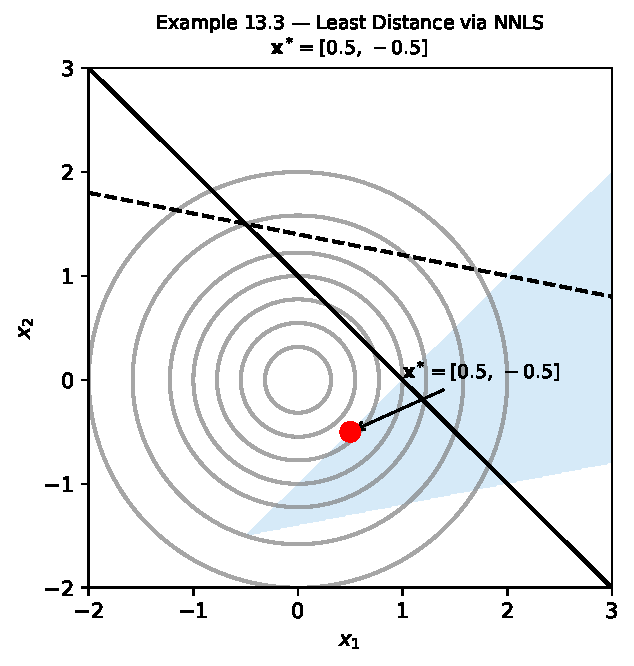
\includegraphics[width=\linewidth]{fig_nnls_demo}
      \end{center}
  \end{columns}
\end{frame}

% =============================================================================
\section{13.5 Solving Nonnegative Least-Squares (NNLS)}
% =============================================================================

\begin{frame}{NNLS: Problem Setup and Partition}
  \begin{block}{Nonnegative Least-Squares (NNLS) --- Eq.~(13.32)}
    \[
      \minimize_{\bx}\; \norm{\bE\bx - \mathbf{f}}
      \qquad \text{subject to}\quad \bx \geq \mathbf{0}
    \]
    where $\bE \in \R^{m\times n}$, $\bx \in \R^n$, $\mathbf{f} \in \R^m$.
  \end{block}

  \textbf{Simplex-inspired partition:} Assign each index $i$ to $\mathcal{B}$ or $\mathcal{V}$:
  \begin{align}
    i \in \mathcal{B} &\implies x_i \geq 0 \quad\text{(inactive constraint)} \tag{13.54}\\
    i \in \mathcal{V} &\implies x_i = 0 \quad\text{(active constraint)} \tag{13.55}
  \end{align}

  \begin{columns}[T]
    \column{0.48\textwidth}
      \textbf{At a solution $\bx^*$:}
      \begin{itemize}
        \item $\mathbf{x}_{\mathcal{V}} = \mathbf{0}$
        \item $\bx^*$ minimizes $\norm{\bE_{\mathcal{B}}\bx - \mathbf{f}}$ over $\mathcal{B}$
        \item Dual variables: $\mu_i \geq 0$ for $i\in\mathcal{V}$, $\mu_i = 0$ for $i\in\mathcal{B}$ with $x_i > 0$
      \end{itemize}

    \column{0.48\textwidth}
      \textbf{KKT conditions at $\bx^*$:}
      \[
        \bmu = \bE^{\top}(\bE\bx^* - \mathbf{f})
      \]
      \begin{itemize}
        \item If $\bmu \geq \mathbf{0}$: optimality confirmed
        \item Else: relax the constraint with most negative $\mu_i$
      \end{itemize}
  \end{columns}
\end{frame}

\begin{frame}{Algorithm 13.4 --- NNLS Solver}
  \begin{block}{Lawson--Hanson Active-Set Algorithm}
    Initialize: $\bx = \mathbf{0}$, $\mathcal{B} = \emptyset$, $\mathcal{V} = \{1,\ldots,n\}$, max $3n$ iterations.
  \end{block}

  \begin{enumerate}
    \item Compute $\bmu = \bE^{\top}(\bE\bx - \mathbf{f})$
    \item \textbf{If} all $\mu_i \geq 0$: \textbf{return} $(\bx, \texttt{true})$  \hfill (KKT satisfied)
    \item Select \textbf{entering index} $q = \arg\min_{i\in\mathcal{V}} \mu_i$ (most negative)
    \item Move $q$ from $\mathcal{V}$ to $\mathcal{B}$; set $\bE_{\mathcal{B}}[:,q] = \bE[:,q]$
    \item \textbf{Inner loop} (while $\mathcal{B} \neq \emptyset$ and $\alpha \neq 1$):
      \begin{enumerate}
        \item $\mathbf{z} = \bE_{\mathcal{B}}^+\mathbf{f}$ \quad (pseudoinverse solve)
        \item If $z_q \leq 0$: remove $q$ back to $\mathcal{V}$; break
        \item $\alpha = \min\left(1,\; \min_{i: z_i < 0, i\in\mathcal{B}} \frac{x_i}{x_i - z_i}\right)$
        \item $\bx_{\mathcal{B}} \leftarrow \bx_{\mathcal{B}} + \alpha(\mathbf{z}_{\mathcal{B}} - \bx_{\mathcal{B}})$
        \item Zero out any $x_i \leq 0$; move those indices back to $\mathcal{V}$
      \end{enumerate}
    \item Update $\bmu \leftarrow \bE^{\top}(\bE\bx - \mathbf{f})$; repeat
  \end{enumerate}

  \begin{block}{Guarantee}
    Every NNLS problem has a solution; this algorithm always terminates.
    Max $3n$ outer iterations.
  \end{block}
\end{frame}

\begin{frame}[fragile]{Python: NNLS Algorithm Implementation}
\begin{lstlisting}[caption={Algorithm 13.4 in Python (Lawson--Hanson active-set method)}]
import numpy as np
from scipy.optimize import nnls as scipy_nnls

def solve_nnls(E, f, max_iter=None):
    """
    NNLS: minimize ||Ex - f|| s.t. x >= 0
    Implements Lawson-Hanson active-set (Algorithm 13.4).
    Returns (x, solved).
    """
    m, n = E.shape
    if max_iter is None:
        max_iter = 3 * n
    x = np.zeros(n)
    mu = -E.T @ f          # initial dual estimate
    P = np.zeros(n, dtype=bool)   # True = active in B
    Ep = np.zeros((m, n))
    q_prev = -1

    for _ in range(max_iter):
        if np.all(P) or np.all(mu >= 0):
            return x, True   # success
        # Choose entering index (most negative mu not in B and != q_prev)
        candidates = [(mu[i], i) for i in range(n) if not P[i] and i != q_prev]
        if not candidates:
            break
        q = min(candidates)[1]
        q_prev = q
        P[q] = True
        Ep[:, q] = E[:, q]
        alpha = 0.0
        while np.any(P) and alpha != 1.0:
            z = np.linalg.pinv(Ep) @ f  # pseudoinverse solve
            if z[q] <= 0:
                mu[q] = 0.0; P[q] = False; Ep[:, q] = 0.0; break
            active = np.where(P)[0]
            ratios = [x[i]/(x[i]-z[i]) if z[i] < 0 else 1.0 for i in active]
            alpha = min(ratios)
            x[P] += alpha * (z[P] - x[P])
            for i in range(n):
                if x[i] <= 0:
                    x[i] = 0.0
                    if P[i]: P[i] = False; Ep[:, i] = 0.0
        mu = E.T @ (E @ x - f)
    return x, False   # too many iterations

# Verify with scipy
E_ex = np.array([[2., 1.], [-4., 3.]])
f_ex = np.array([5., 5.])
x_manual, _ = solve_nnls(E_ex, f_ex)
x_scipy, _  = scipy_nnls(E_ex, f_ex)
print(f"Manual: {x_manual.round(4)}")
print(f"SciPy:  {x_scipy.round(4)}")
\end{lstlisting}
\end{frame}

\begin{frame}{NNLS Algorithmic Progression --- Example 13.4}
  \[
    \bE = \begin{bmatrix}2.0 & 1.0\\-4.0 & 3.0\end{bmatrix}
  \]

  \begin{center}
    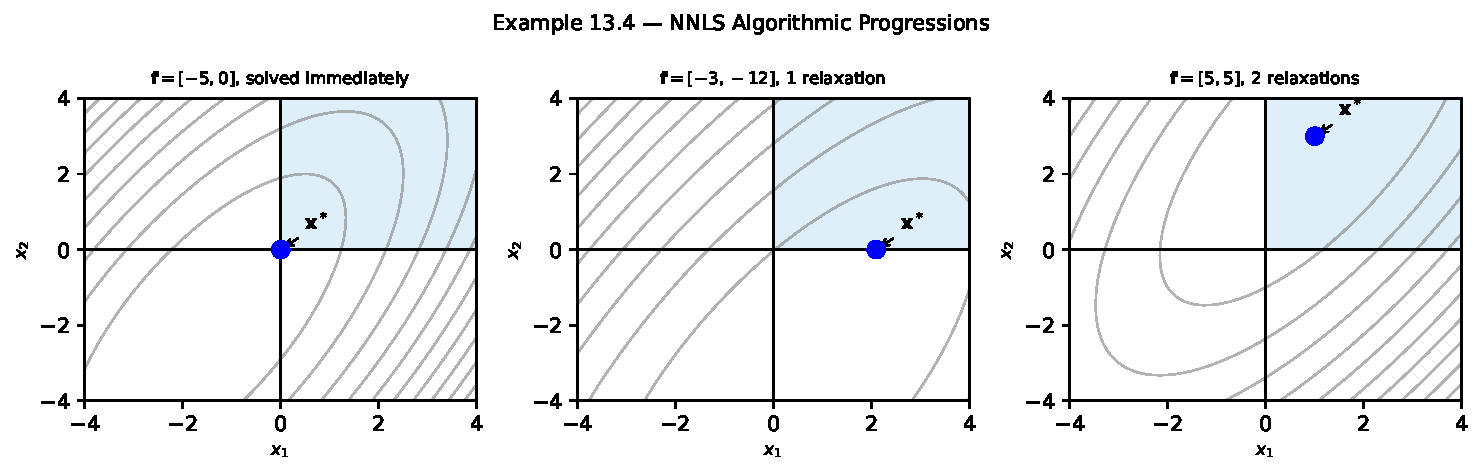
\includegraphics[width=0.88\linewidth]{fig_nnls_progression}
  \end{center}

  \begin{itemize}
    \item $\mathbf{f} = [-5, 0]$: unconstrained minimizer already in $\bx\geq\mathbf{0}$ \textrightarrow\ 0 relaxations
    \item $\mathbf{f} = [-3, -12]$: 1 constraint relaxation needed
    \item $\mathbf{f} = [5, 5]$: 2 constraint relaxations needed
  \end{itemize}
\end{frame}

\begin{frame}{KKT Proof of NNLS Optimality}
  \textbf{Goal:} Show that $\bx^*$ from Algorithm 13.4 satisfies KKT for the LDP.

  \begin{columns}[T]
    \column{0.50\textwidth}
      \textbf{Step 1: Feasibility.}
      From KKT, gradient of NNLS objective is balanced by constraints:
      \[
        \mathbf{0} \leq \bE^{\top}\mathbf{r} = [\bG\;\bh]\begin{bmatrix}\bx^*\\-1\end{bmatrix}(-r_{n+1})
        = (\bG\bx^* - \bh)\norm{\mathbf{r}}^2 \tag{13.45}
      \]
      This shows $\bG\bx^* \geq \bh$. \checkmark

    \column{0.46\textwidth}
      \textbf{Step 2: Stationarity.}
      \begin{align}
        \bx^* - \bG^{\top}\bmu &= \mathbf{0} \tag{13.48}\\
        \bx^* &= \bG^{\top}\bmu \tag{13.49}
      \end{align}
      with $\bmu = \mathbf{y}^*\norm{\mathbf{r}}^{-2} \geq \mathbf{0}$.

      \textbf{Step 3: Complementary slackness.}
      $y_i^*$ is zero for inactive constraints.
  \end{columns}

  \begin{alertblock}{Conclusion}
    We have a primal-dual pair $(\bx^*, \bmu^*)$ satisfying all KKT conditions for a
    convex problem $\Rightarrow$ $\bx^*$ is \textbf{globally optimal}.
  \end{alertblock}
\end{frame}

% =============================================================================
\section{13.6 Dual Certificates}
% =============================================================================

\begin{frame}{Dual Problem for QP}
  Consider the general QP (13.1) with positive-definite $\bQ$:
  \[
    \minimize_{\bx}\; \tfrac{1}{2}\bx^{\top}\bQ\bx + \bq^{\top}\bx
    \quad \text{s.t.}\quad \bC_{\text{LE}}\bx \leq \bd_{\text{LE}},\; \bC_{\text{EQ}}\bx = \bd_{\text{EQ}}
  \]

  \begin{block}{Lagrangian --- Eq.~(13.58)--(13.60)}
    \[
      \mathcal{L}(\bx, \bmu, \blambda)
      = \tfrac{1}{2}\bx^{\top}\bQ\bx + \mathbf{e}^{\top}\bx + f
    \]
    where $\mathbf{e} = \bq + \bC_{\text{LE}}^{\top}\bmu + \bC_{\text{EQ}}^{\top}\blambda$ and
    $f = -\bmu^{\top}\bd_{\text{LE}} - \blambda^{\top}\bd_{\text{EQ}}$.
  \end{block}

  \begin{block}{Dual Function --- Eq.~(13.61)--(13.63)}
    Minimize $\mathcal{L}$ over $\bx$: gradient zero $\Rightarrow$ $\bx^* = -\bQ^{-1}\mathbf{e}$
    \[
      \mathcal{D}(\bmu\geq\mathbf{0}, \blambda)
      = -\tfrac{1}{2}\mathbf{e}^{\top}\bQ^{-1}\mathbf{e} + f
    \]
  \end{block}

  \begin{block}{Dual Problem --- Eq.~(13.64)}
    \[
      \maximize_{\bmu,\blambda}\; -\tfrac{1}{2}\mathbf{e}^{\top}\bQ^{-1}\mathbf{e} + f
      \qquad \text{subject to}\quad \bmu \geq \mathbf{0}
    \]
    Slater's condition $\Rightarrow$ \textbf{zero duality gap}: $f(\bx^*) = \mathcal{D}(\bmu^*, \blambda^*)$.
  \end{block}
\end{frame}

\begin{frame}{Dual Certificates --- Verifying Optimality}
  \begin{center}
    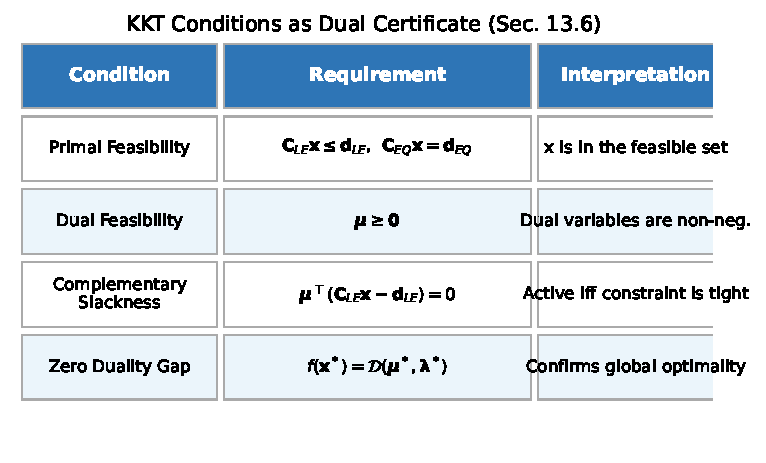
\includegraphics[width=0.80\linewidth]{fig_dual_certificate}
  \end{center}

  \begin{block}{Strong Duality (Slater's Condition holds)}
    If the QP is feasible and strictly feasible (Slater), then at the optimum:
    \[
      f(\bx^*) = \mathcal{D}(\bmu^*, \blambda^*)
      \quad\Longleftrightarrow\quad\text{primal-dual pair is optimal}
    \]
  \end{block}

  \begin{itemize}
    \item Dual certificate: verify $(\bx^*, \bmu^*, \blambda^*)$ satisfies all KKT conditions
    \item Dual problem may be \emph{easier} to solve than the primal in some cases
    \item NNLS solution provides an implicit dual certificate (Section 13.5)
  \end{itemize}
\end{frame}

\begin{frame}[fragile]{Python: Dual Certificate Verification}
\begin{lstlisting}[caption={Check KKT conditions for a QP solution using NumPy}]
import numpy as np

def verify_kkt(Q, q, C_LE, d_LE, x_star, mu_star, tol=1e-6):
    """
    Verify KKT conditions for QP:
      min (1/2)x^T Q x + q^T x  s.t.  C_LE x <= d_LE
    Parameters: primal x_star, dual mu_star (>= 0)
    """
    # 1. Primal feasibility
    primal_feas = np.all(C_LE @ x_star <= d_LE + tol)

    # 2. Dual feasibility
    dual_feas = np.all(mu_star >= -tol)

    # 3. Stationarity:  Q x + q + C_LE^T mu = 0
    stationarity = np.linalg.norm(Q @ x_star + q + C_LE.T @ mu_star) < tol

    # 4. Complementary slackness:  mu_i * (C_LE x - d_LE)_i = 0
    slack = C_LE @ x_star - d_LE          # should be <= 0
    comp_slack = np.abs(mu_star @ slack) < tol

    return {'primal_feasible': primal_feas,
            'dual_feasible':   dual_feas,
            'stationary':      stationarity,
            'comp_slack':      comp_slack}

# Dual objective value D(mu, lambda)
def dual_value(Q, q, C_LE, d_LE, mu, lam=None, C_EQ=None, d_EQ=None):
    e = q + C_LE.T @ mu
    if C_EQ is not None and lam is not None:
        e = e + C_EQ.T @ lam
    f = -mu @ d_LE
    if d_EQ is not None and lam is not None:
        f = f - lam @ d_EQ
    return -0.5 * e @ np.linalg.solve(Q, e) + f
\end{lstlisting}
\end{frame}

% =============================================================================
\section{Summary \& Exercises}
% =============================================================================

\begin{frame}{Chapter 13 Summary}
  \begin{block}{Key Concepts}
    \begin{enumerate}
      \item \textbf{Quadratic programs} have quadratic objectives and linear constraints.
      \item A \textbf{convex} QP (positive-definite $\bQ$) is equivalent to a least-squares problem.
      \item \textbf{Unconstrained least squares} is solved exactly via the \emph{pseudoinverse} $\bA^+\bb$.
      \item A \textbf{general least-squares} problem converts to a LS with linear inequalities via LQ decomposition.
      \item LS with inequalities converts to a \textbf{least distance program} (LDP).
      \item An LDP converts to a \textbf{nonneg.\ least-squares} (NNLS) problem.
      \item NNLS is solved by the \textbf{Lawson--Hanson active-set} method (Alg.~13.4).
      \item \textbf{Dual certificates} (KKT conditions + zero duality gap) verify global optimality.
    \end{enumerate}
  \end{block}

  \begin{center}
    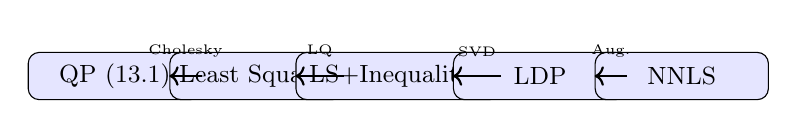
\begin{tikzpicture}[node distance=1.8cm, every node/.style={draw, rounded corners, fill=blue!10, minimum width=2.2cm, minimum height=0.6cm, font=\small}]
      \node (qp) {QP (13.1)};
      \node (ls) [right of=qp] {Least Squares};
      \node (lsi) [right of=ls, minimum width=2.6cm] {LS+Inequalities};
      \node (ldp) [right of=lsi] {LDP};
      \node (nnls) [right of=ldp] {NNLS};
      \draw[->, thick] (qp) -- node[draw=none, fill=none, above, font=\tiny]{Cholesky} (ls);
      \draw[->, thick] (ls) -- node[draw=none, fill=none, above, font=\tiny]{LQ} (lsi);
      \draw[->, thick] (lsi) -- node[draw=none, fill=none, above, font=\tiny]{SVD} (ldp);
      \draw[->, thick] (ldp) -- node[draw=none, fill=none, above, font=\tiny]{Aug.} (nnls);
    \end{tikzpicture}
  \end{center}
\end{frame}

\begin{frame}{Selected Exercises}
  \begin{block}{Exercise 13.1}
    Are NNLS problems always feasible?\\
    \textit{Yes}: $\bx \geq \mathbf{0}$ is always satisfiable (e.g., $\bx = \mathbf{0}$).
  \end{block}

  \begin{block}{Exercise 13.2}
    Are LDPs always feasible?\\
    \textit{No}: $\bG\bx \geq \bh$ may be empty. Example:
    $\mathbf{1}^{\top}\bx \geq 1$ and $-\mathbf{1}^{\top}\bx \geq 1$ simultaneously.
  \end{block}

  \begin{block}{Exercise 13.3}
    Do LDPs have unique solutions?\\
    \textit{Yes}: Suppose two optimal solutions $\mathbf{a}, \mathbf{b}$ with $\norm{\mathbf{a}} = \norm{\mathbf{b}}$.
    Then $\mathbf{c} = \tfrac{1}{2}(\mathbf{a}+\mathbf{b})$ is feasible and $\norm{\mathbf{c}} < \norm{\mathbf{a}}$ (strict convexity) --- contradiction.
  \end{block}

  \begin{block}{Exercise 13.5}
    WLOG, $\bQ$ can be assumed symmetric:
    $\bx^{\top}\bQ\bx = \bx^{\top}\bQ_{\text{sym}}\bx$ where $\bQ_{\text{sym}} = \tfrac{1}{2}(\bQ + \bQ^{\top})$,
    since the antisymmetric part $\bQ_{\text{anti}} = -\bQ_{\text{anti}}^{\top}$ satisfies
    $\bx^{\top}\bQ_{\text{anti}}\bx = 0$ for all $\bx$.
  \end{block}
\end{frame}

\begin{frame}{Exercise 13.6 --- QP $\equiv$ Least Squares}
  \begin{block}{Show: $\minimize_\bx \norm{\bU\bx + \bU^{-\top}\bq} \equiv \minimize_\bx \frac{1}{2}\bx^{\top}\bQ\bx + \bq^{\top}\bx$}
  \end{block}

  \begin{align*}
    \arg\min_\bx \norm{\bU\bx + \bU^{-\top}\bq}
    &= \arg\min_\bx \norm{\bU\bx + \bU^{-\top}\bq}^2\\
    &= \arg\min_\bx (\bU\bx + \bU^{-\top}\bq)^{\top}(\bU\bx + \bU^{-\top}\bq)\\
    &= \arg\min_\bx \bx^{\top}\bU^{\top}\bU\bx + \bq^{\top}\bU^{-1}\bU\bx
       + \bx^{\top}\bU^{\top}\bU^{-\top}\bq + \bq^{\top}\bU^{-1}\bU^{-\top}\bq\\
    &= \arg\min_\bx \bx^{\top}\bQ\bx + 2\bq^{\top}\bx + \bq^{\top}\bQ^{-1}\bq\\
    &= \arg\min_\bx \tfrac{1}{2}\bx^{\top}\bQ\bx + \bq^{\top}\bx
  \end{align*}

  (constant $\bq^{\top}\bQ^{-1}\bq$ dropped; factor of 2 absorbed into $\bq^{\top}\bx$.)
\end{frame}

\begin{frame}[fragile]{Complete Python Pipeline --- Example 13.1}
\begin{lstlisting}[caption={Full QP solution pipeline in Python using scipy.optimize.minimize}]
import numpy as np
from scipy.optimize import minimize, LinearConstraint

# Example 13.1: minimize ||Ax - b|| s.t. 2x1 - x2 >= 2, x1 - 3x2 <= 4
A = np.array([[2., 1.], [-4., 3.]])
b_vec = np.array([1., 2.])

# Quadratic form: Q = A^T A,  q = -A^T b
Q = A.T @ A
q = -A.T @ b_vec

def objective(x):
    return 0.5 * x @ Q @ x + q @ x

def gradient(x):
    return Q @ x + q

# Constraints: 2x1 - x2 >= 2  =>  [2, -1] x >= 2
#              x1 - 3x2 <= 4  =>  -x1 + 3x2 >= -4
C = np.array([[ 2., -1.],   # 2x1 - x2 >= 2
              [-1.,  3.]])   # x1 - 3x2 <= 4 (negated)
d = np.array([2., -4.])

constraint = LinearConstraint(C, lb=d, ub=np.inf)

result = minimize(objective, np.zeros(2), jac=gradient,
                  method='SLSQP', constraints={'type': 'ineq',
                  'fun': lambda x: C @ x - d, 'jac': lambda x: C})
print(f"Optimal x*  = {result.x.round(4)}")  # [1.4, 0.8]
print(f"Objective   = {result.fun:.6f}")
print(f"Success     = {result.success}")
\end{lstlisting}
\end{frame}

% -- Final slide ---------------------------------------------------------------
\begin{frame}{Conclusion}
  \begin{center}
    {\Large Chapter 13: Quadratic Programming}\\[1em]
    {\large Algorithms for Optimization, 2nd ed.}\\[0.5em]
    Kochenderfer \& Wheeler, MIT Press, 2026
  \end{center}

  \vspace{1em}
  \begin{columns}[T]
    \column{0.48\textwidth}
      \textbf{What we covered:}
      \begin{itemize}
        \item QP formulation and geometry
        \item Unconstrained LS via pseudoinverse
        \item Equality/inequality elimination
        \item Least Distance Programs
        \item NNLS: Lawson--Hanson algorithm
        \item Dual certificates \& KKT
      \end{itemize}

    \column{0.48\textwidth}
      \textbf{Python tools used:}
      \begin{itemize}
        \item \texttt{numpy.linalg.pinv} --- pseudoinverse
        \item \texttt{scipy.linalg.lstsq} --- least squares
        \item \texttt{scipy.optimize.nnls} --- NNLS
        \item \texttt{scipy.optimize.minimize} (SLSQP) --- general QP
        \item \texttt{scipy.linalg.svd} --- SVD decomposition
      \end{itemize}
  \end{columns}
\end{frame}

\end{document}
